% プロジェクト学習中間報告書書式テンプレート ver.1.0 (iso-2022-jp)

% 両面印刷する場合は `openany' を削除する
\documentclass[openany,11pt,papersize]{jsbook}
  
  % 報告書提出用スタイルファイル
  \usepackage[final]{funpro}%最終報告書
  %\usepackage[middle]{funpro}%中間報告書

  % 画像ファイル (EPS, EPDF, PNG) を読み込むために
  \usepackage[dvipdfmx]{graphicx,color}
  
  % ファイル分割のためのパッケージ
  \usepackage{subfiles}
  
  % ここから -->
  \usepackage{calc,ifthen}
  \newcounter{hoge}
  \newcommand{\fake}[1]{\whiledo{\thehoge<70}{#1\stepcounter{hoge}}%
    \setcounter{hoge}{0}}
  % <-- ここまで 削除してもよい
  
  % 年度の指定
  \thisYear{2017}
  
  % プロジェクト名
  \jProjectName{ビーコンIoTで函館のまちをハックする}
  
  % [簡易版のプロジェクト名]{正式なプロジェクト名}
  % 欧文のプロジェクト名が極端に長い(2行を超える)場合は、短い記述を
  % 任意引数として渡す。
  %\eProjectName[Making Delicious curry]{How to make delicious curry of Hakodate}
  \eProjectName{Leverage the Beacon IoT in Hakodate Real Downtown for Our Smarter Life}
  
  
  % <プロジェクト番号>-<グループ名>
  \ProjectNumber{8-A}
  
  % グループ名
  \jGroupName{Hako-B}
  \eGroupName{Hako-B}
  
  % プロジェクトリーダ
  \ProjectLeader{1015253}{橋場保鷹}{Hodaka~Hashiba}
  
  % グループリーダ
  \GroupLeader  {1015053}{佐藤秀輔}{Shusuke~Sato}
  
  % メンバー数
  \SumOfMembers{4}
  % グループメンバ
  \GroupMember  {1}{1015050}{北原康太}{Kota~Kitahara}
  \GroupMember  {2}{1015053}{佐藤秀輔}{Shusuke~Sato}
  \GroupMember  {3}{1015157}{小笠原瑠奈}{Runa~Ogasawara}
  \GroupMember  {4}{1015204}{小島雄士}{Yuji~Kojima}
  
  % 指導教員
  \jadvisor{松原克弥,藤野雄一,鈴木恵二,奥野拓}
  % 複数人数いる場合はカンマ(,)で区切る。カンマの前後に空白は入れない。
  \eadvisor{Katsuya~Matsubara,Yuichi~Fujino,Keiji~Suzuki,Taku~Okuno}
  
  % 論文提出日
  \jdate{2017年7月26日}
  \edate{July~26, 2017}
  
  \begin{document}
  %
  % 表紙
  \maketitle
  
  %前付け
  \frontmatter
  
  % 和文概要
  \begin{jabstract}
  
  % プロジェクト全体の日本語概要
  \subfile{common/common-jabstract}
  
% プロジェクト全体の日本語概要

本グループでは、函館バスの利用がうまくできていないという問題点に目をつけ函館バスを快適に利用することができるアプリケーションの開発を行うこととした。
問題点を下に、私達はどのようにビーコンを用いてバス利用を改善していくかを担当の教員の方からレビューを受けながらアイディアを固めた。
そのアイディアなどを下にサービス設計を行い、後期の活動から開発をするための準備を行った。
7月14日に行われた中間発表会ではビーコンの特性を活かしきれていないのではないかとの指摘もあり、よりビーコンの強みを活かした設計が必要だという課題が見つかった。

% 和文キーワード
\begin{jkeyword}
ビーコン, フィールドワーク, 函館バス, アプリケーション, 設計
\end{jkeyword}
\bunseki{佐藤秀輔}
\end{jabstract}

%英語の概要
\begin{eabstract}

% プロジェクト全体の英語概要
 \subfile{common/common-eabstract}
 % グループの英語概要

In this group, we decided to focus on the problem that utilization of Hakodate bus was not done well and to develop services.
From that point, we accepted reviews from teachers in charge how to improve the use of the bus by using beacons while consolidating ideas.
We designed the service based on the idea etc. and prepared for development from the latter term activities.
In the interim presentation held on July 14th, there was a case that the characteristics of the beacon could not be fully utilized, and a problem was found that it is necessary to design with the advantage of Beacon more.

% 英文キーワード
\begin{ekeyword}
Beacon, Fieldwork, Hakodate's Bus, Application, Design
\end{ekeyword}
\bunseki{佐藤秀輔}
\end{eabstract}

  
  \tableofcontents% 目次
  
  
  \mainmatter% 本文のはじまり
  
  % プロジェクト共通の項目
  \subfile{common/common-chapters}
  
  
  
  % グループごとの項目
  
  \chapter{本グループについて}


\section{\midorfin{函館バスの現状と従来のIT利用例}{背景}}

函館市の交通手段として車、市電、バスなどがある。その中でもよく活用する移動手段としてバスがある。バスは気軽に利用でき、車を持っていない人は必然的に利用回数が多くなる。また、バスの時刻表やバスの接近情報を表示する既存のウェブサイトやアプリケーションが存在しているがGPSを用いているため、局所的なバスやバス停の位置の把握に誤差が生じる場合がある。

\bunseki{小島雄士}

\section{函館バスが抱える問題点}

フィールドワークやブレーンストーミングなどの話し合いをした結果、バス停についての問題点、バスの情報を発信しているウェブサイトについての問題点が見つかった。\\
まず、バス停についての問題点は2つ見つかった。
1つ目の問題点は、バスは函館に馴染んでいるが、函館のバス停の中にはわかりにくいものも多いという点である。例えば、「五稜郭」というバス停は同じ名前のバス停が近くに八つ存在している(図3.1)。
これは観光で初めて利用した人にとっても地元住民にとっても分かりにくい。
また、路線が完全に一致しているが往と復で別系統となっている路線も存在し、系統番号だけでは判断できず、バスの乗り間違え、目的のバスがどこに止まるか分からず乗れない、といった問題があげられる。
2つ目の問題点は、似たような名前のバス停が多い点である。前、入口、裏などがあり分かりにくい停留所も存在している。
このためバス停の名前を把握していない人にとって、目的地へ行くためにどこで降りればよいのか分かりにくい、という問題があげられる。\\
次に、バスの情報を発信しているウェブサイトの問題点は2つ見つかった。
まず1つ目の問題点は、バスの接近情報が正確ではない時がある、という点である。
理由は、バスに搭載されている機器がGPS衛星と定期的に通信するため、バスの位置を即位するときに誤差が生じるからである。
さらに大雨の時、渋滞の時、冬に雪が降っている時などは接近情報が「調整中」となり正確な情報を取得できない場合がある。
2つ目の問題点としては、ウェブサイトを利用して目的地を検索することが難しい点である。
あるページはバス停の名前が分からない人のためにマップから検索することができる仕組みとなっている。
しかしマップから選択する時、広範囲な地域選択しかできない。
選択後は目的地候補名が一覧表示されるが、その目的地一覧にない場所へ行きたい時は利用することができない。

\bunseki{小島雄士}

\section{目的}\label{sec:gaiyou}
本グループでは「バス、バス停にビーコンを設置し、函館バスの乗降のミスを少なくする」ことを目的とした。
3.2項であげたように本グループはバス停留所やバスの情報を発信しているウェブサイトについて、いくつかの問題点を発見した。
これらの問題点を解決するために、函館のバスをより使いやすくするアプリケーションの開発を行う。
特に、函館のバスを初めて利用した人にも使いやすいようなアプリケーションを目指す。

\bunseki{小島雄士}

\begin{figure}[htbp]
  \begin{center}
    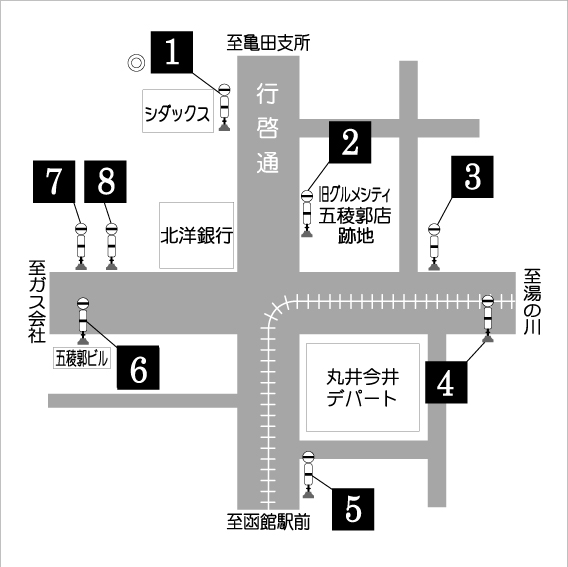
\includegraphics[clip,width=7.0cm]{img/14007.jpg}
    \caption{五稜郭バス停}
    \label{fig:goryo}
  \end{center}
\end{figure}

\chapter{Hako-Bについて}

\section{Hako-bの概要}
Hako-bは、ターゲットを函館バスを初めて使う観光客へ向けたサービスである。
初めて函館に来た観光客でも迷うことなく函館のバスに乗ることができれば、地元の方にも分かりやすいサービスとなるため、観光客にターゲットを当てた。
函館バスの分かりづらい点として、3.2項であげた問題のほか、路線が完全に一致しているが往と復で別系統となっている路線も存在し、系統番号だけでは判断できない。
それらを解決するために私達はHako-bを提案する。
Hako-bのサービスの概要はバス、バス停にビーコンを設置し、バス利用者が乗車予定のバスの系統番号や行き先情報を既存のバスロケーションシステムや時刻表を見なくても乗車できることを目的としたアプリケーションサービスである。
\bunseki{北原康太}


\section{Hako-bの機能}
観光客がHako-bアプリを起動すると、GPSを用いてマップから降車位置を選択でき、降車位置決定後、現在位置の周りにあるバス停を選択することができる。
その後、現在位置から乗車予定のバス停までの経路表示をする。乗車予定のバス停に近づくと、バス停に設置してあるビーコンから「乗車予定のバス停に近づきました。」というPush通知が送られ、近くにバス停が複数ある場所でも、迷わずに乗車するバス停にたどり着くことができる。
そして、バス停に乗車予定のバスが到着した際には「乗車するバスが到着しました。バスに乗ってください。」というPush通知が送られて、複雑な系統番号や降車地が書かれていないバスでも間違うことなく正しいバスに乗れる。
\bunseki{北原康太}

\section{サービス設計}

\subsection{システム概要}
本システムは、バス、バス停に設置されたビーコンにより、そのバス、バス停の正誤判定をするというシステムである。
主な機能としては、目的のバス、バス停に近づいた際にPush通知を送るというものである。
また、Push通知を送るだけでなく、近くのバス停をマップから選択し、時刻表などを確認することができ、利用者が簡単にバスの情報を集めることができる。

\bunseki{佐藤秀輔}

\subsection{機能一覧}
本アプリケーションの機能は、主に5種類の機能がある。以下にそれぞれの機能について述べる。
\begin{enumerate}

\item Bluetooth通知機能\\
ユーザの持っている端末にてBluetoothがONになっているか検知する。ONになっていない場合は通知を送りBluetoothをONにするように促す。
\item バス停の選択\\
ユーザがマップよりバス停を選択し乗るバスを確定させる。
\item バスの時刻表表示機能\mbox{}\\
マップ上でバス停を選択し、その選択されたバス停の時刻表を表示する。
\item 通知機能\mbox{}\\
ユーザの目的のバス、バス停に設置してあるビーコンの電波範囲内に入った際に通知を行う。
\item 案内機能\mbox{}\\
ユーザが設定したバス停情報を元に、乗車予定のバス停までの道案内をする。

\end{enumerate}

\bunseki{佐藤秀輔}

\subsection{ユースケース}
システムとユーザ間でどのような処理が必要になるのか確認するためにユースケースを作成した。
それを元にユースケース図を作成した(図4.1)。
アクターである観光者はアプリを起動し、目的地、現在地付近のバス停を選択する。
選択したのち、ユーザが選択したバス停のビーコンの範囲内に入るとPush通知を受け取る。
その後、目的地まで向かうバスに設置されたビーコンの範囲内に入るとPush通知を受け取る。

\begin{figure}[htbp]
  \begin{center}
    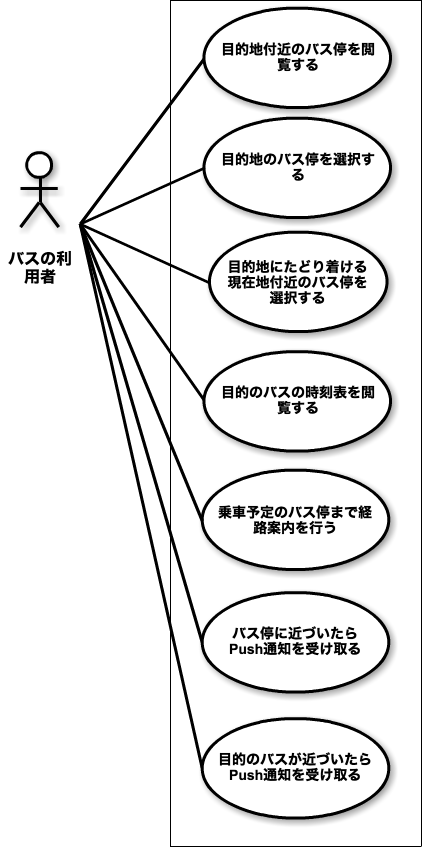
\includegraphics[clip,width=7.0cm]{img/usecase.png}
    \caption{ユースケース図}
    \label{fig:usecase}
  \end{center}
\end{figure}
\bunseki{佐藤秀輔}


\chapter{中間発表}

\section{発表形式}
始めにメインポスターの発表を5分間行った後、聞き手には3つのサブポスターのどれかを選んでもらいそれぞれ発表を聞いてもらった。
Hako-Bのポスターセッションでは前半と後半それぞれ2人ずつに分かれて発表を行った。
一人は概要、システム構成、今後の予定を話し、もう一人はHako-Bについてを話した。

\bunseki{小笠原瑠奈}

\section{発表内容}
始めに、概要を説明した。
まず、Hako-Bを提案するに至った問題点を実際のバス停の例と画像を用いて提示した。
1つ目は同じバス停名が近くに複数存在すること、2つ目は似たような名前のバス停が存在すること、3つ目は目的地に行くためのバスの系統がわかりづらいことだった。
その後、先に述べた問題から生じるミスを解消することを目的とした。次にHako-Bの機能説明をした。
まず、アプリの特徴を箇条書きで大まかに示した。
特徴は3つあり、1つ目は利用者が設定したバス停までの道案内を GPS を用いて行うこと、2つ目はバス停に設置されたビーコンから受けた電波によってバス停への接近を利用者に通知すること、3つ目はバスの車内に設置されたビーコンから受けた電波によってバスの到着を通知することである。
その後、処理フローでイラストやスマホ画面などの画像を用いてアプリの機能を具体的に説明した。
次に、システム構成の説明を行った。
最後に、今後の予定を3つ示した。
1つ目は設計を基にプロトタイプを作成すること、2つ目は模擬バス,模擬バス停による実証実験を行うこと、3つ目はテストで出た問題の改善を行うことである。
以上がポスター発表の内容となる。

\bunseki{小笠原瑠奈}

\section{レビュー内容}

\subsection{発表方法についての評価と反省}
発表技術に関して、プラスの意見として
\begin{itemize}

\item 身振り手振りがあって良い
\item 発表が分かりやすかった

\end{itemize}
などが挙げられ、聞き手に内容を上手く伝えることができたと分かる。以上から発表技術に問題はなかったと言える。
マイナスの意見としては
\begin{itemize}

\item 声が聞き取りづらい
\item ポスターのレイアウトが意味不明
\item 画面遷移図が小さい
\item 図に少し説明を入れると良い

\end{itemize}
などが挙げられた。平均評価は7であった。
以上から、発表する際の各グループの配置や向きを見直す必要があること、ポスターのレイアウトを読み進めやすいものにすること、アプリ画面のテキストをポスター用に大きくすること、図を見やすくして説明を付けることが改善点として挙げられる。

\bunseki{小笠原瑠奈}

\subsection{発表内容についての評価と反省}
発表内容に関しては、プラスの意見として
\begin{itemize}

\item 問題の着目点が良い
\item アプリのニーズは高い
\item 実際に欲しい

\end{itemize}
などが挙げられ、提案に対する聞き手のニーズが高いことがうかがえた。マイナスの意見としては、
\begin{itemize}

\item プロトタイプもできていないので課題が山積み
\item 内容の検討がたりない
\item ビーコンの利点をうまく使いこなせていない。もっと他にも良い活用法があるかもしれない
\item バス停名が分からない人にはどうするのか
\item 計画を具体的に詰めたら良い

\end{itemize}
などが挙げられ、提案システムの問題点や今後の予定が詳細に決められていないことに指摘を受けた。
平均評価は7であった。
以上から、今後出来るだけ早い段階からプロトタイプを作る必要があること、様々なアクターを想定したユースケースを再検討すること、今後の計画を詳細に決めることが改善点として挙げられる。
また、「バス停名が分からない人にはどうするのか」という指摘に対しては、ユーザーが目的地を入力するとマップ上から推奨される降車地と乗車地を選択できるというアプリの機能が解決策となる。
しかし、これは展望であり、実装予定の機能としてはポスターに載せていなかったので説明不足であったと反省する。

\bunseki{小笠原瑠奈}


\chapter{開発準備}
\section{開発に用いたツールとその経緯}
\subsection{Xcode}
今回のアプリ開発ではAndroid、iOSの両方の開発をすることが難しいためiOSのアプリ開発を行うこととした。
そのためアプリ開発には、Apple社が開発したXcodeと言うソフトウェアを使用して開発することにした。
開発言語はSwiftを使用した。
使用したバージョンはXcode8.3、Swift3.0の環境で開発をした。
XcodeにはInterfaceBuilderという機能があり実際にコードを書かなくても視覚的にUIを作成する機能があり、リファレンスなど充実しているため開発ツールにXcodeを選択した。
また、Xcode上でシミュレータを起動し実際にiPhoneで動かしているかのようなデバック機能があるため実際にiPhoneを持っていたりしなくても現在のコードを確認できるというメリットも有る。

\bunseki{佐藤秀輔}

\subsection{Git/GitHub}
ソースコードのバージョン管理ツールとしてGit/GitHubを使用した。
Gitは分散型のバージョン管理システムの一つであり、すべてのファイルの変更履歴を含む完全なリポジトリの複製を保存できるというものである。
その為、一度編集したファイルを元に戻すことやどのような編集が行われたのか表示することが可能となる。
リポジトリにはネットワーク上に保存されているリモートリポジトリと、メンバーそれぞれのPC内に保存されているローカルリポジトリの2種類がある。
リモートリポジトリではメンバーそれぞれのファイルの変更履歴を保存し確認、共有することができる。
GitHubとはリモートリポジトリを提供するサービスの一つである。
これにより、複数のメンバー間でスムーズにファイルを共有し開発することが可能となった。

\bunseki{佐藤秀輔}

\subsection{Adobe Illustrator}
ポスターの作成にはAdobe Illustratorを使用した。
IllustratorはAdobe Systemsが販売しているベクター編集ツールで、イラストやポスターなど作成することができるツールである。

\bunseki{佐藤秀輔}

\section{環境構築}
Xcodeを使用するためにまずはAppleIDの作成が必要だったため個人が持っているアカウントもしくは開発のためにAppleアカウントを作成を行った。
開発の環境としてはXcodeのインストールを行うことで整うためXcodeのインストールを行った。
GitHubに関しては、リモートリポジトリに機能の追加、バグの修正などの種類ごとにブランチを作成し、そこへプッシュするようにした。
developなどの開発用のブランチを作成せずにmasterにマージする際にテストを行い問題がないかレビューを行いmasterにマージをするという手法で行った。
masterにマージする際にレビューを徹底することでmasterのファイルでバグが起きないようにすることができる。

\bunseki{佐藤秀輔}

\section{夏休みの活動}
メンバー全員でiOSのアプリ開発の経験がある人が1人しかいなかった。
その為、夏休み中にアプリ開発の基礎的な知識を学習できるような資料の作成をしてもらった。
その際のプログラムの教材として
\begin{itemize}

\item Swiftの基礎知識
\item Hello Worldのプログラム作成
\item TableViewを用いたアプリの作成

\end{itemize}
の3つを題材として基礎的な知識について学習を行った。

\bunseki{佐藤秀輔}


\chapter{成果発表}
\section{発表形式}
始めにプロジェクト全体の発表をスライドで 5 分間行った後、聞き手に 3 つのサブポスターのどれかを選んでもらい発表を聞いてもらった。
Hako-B のポスターセッションは中間発表と同じ形式で、発表者の組み合わせも同じであったが、同時にアプリのデモを行った。
一人は問題、Hako Bについて、アプリの使用フロー、学び、展望を話し、もう一人はアプリの機能について実際にアプリを動かして説明した。
デモではアプリがバス停・バスのビーコンを検知することに重点を置き、アプリを動かす方がバス停のビーコンを持ち、もう一人がバスのビーコンを動かすことでプッシュ通知が来る様子を見せた。

\bunseki{小笠原瑠奈}

\section{発表内容}
まず概要において、アプリを開発するに至った背景として、「初めて函館に来た人はバス停名・位置が分かりづらい」、「函館では同じまたは似たような名前のバス停が複数ある」、「目的地に行くためのバスの系統が分かりづらい」、以上の3点を函館バスの問題点であると、例えを交えながら提示した。
その後、提示した問題を解決するために開発したという流れでHako Bとはどのようなアプリなのかを簡潔に説明した。
次にアプリの使用フローを軽く説明した後、分かりやすいよう実際にアプリのデモプレイで、マップから乗車地・降車地を選択した後、次の画面で時刻表をタップすると乗車地までの経路が表示されるという流れを軽く示した。
乗車地・降車地選択の画面では検索フォームに「赤川」と入力すると「赤川」が含まれるバス停だけが表示される様子も見せた。
そして「はこだて未来大学」を想定したビーコンをスマホに近づけると「バス停が近くにあります」、違うビーコンを近づけると「違うよ!」と通知され、バスを想定したビーコンが近づくと「バスが到着しました」と通知される様子を見せた。
最後に、後期の活動を経ての学びとして、「Swift での iOS アプリ開発の流れを学んだ」、「Beacon を用いた局所的な位置情報の利用法を学んだ」の2点と、今後の展望として、「正確なバス遅延時間の表示」、「乗り換えも考えたルートの表示」の2点を提示した。

\bunseki{小笠原瑠奈}

\section{レビュー内容}
\subsection{発表方法についての評価と反省}
発表方法に関して、プレゼンに関するプラスの意見として
\begin{itemize}

\item 具体的なシチュエーションでの説明がわかりやすかった。
\item とても効果的なプレゼンが出来ていました。
\item 詳細をしっかり説明してくれている。
\item 詳細をしっかり説明してくれている。
\item 発表する速さが程度良い感じです。

\end{itemize}

などがあった。また、ポスターに関しては
\begin{itemize}

\item ポスターの図が分かりやすかった
\item と内容をまとめられていたため分かりやすかった。

\end{itemize}

などがあり、デモに関しては
\begin{itemize}

\item 発表技術について、体験ができて、理解しやすかった。
\item デモを行っていてわかりやすい。大きめのディスプレイを使っていてわかりやすかった。

\end{itemize}

などの意見をいただいた。次にマイナスの意見に関しては、
\begin{itemize}

\item 少し声が聞き取りにくかった。
\item 声が小さく聞き取りづらかった。
\item パネルセッションなのでパネルかくさない方がよいのでは?

\end{itemize}
など声の通りに対する意見を多くいただいた。
以上から、内容を説明する流れやポスター、デモは高評価であったことから分かりやすく、効果的であったと思われるが声量や動きに問題があったと言える。
平均評価は7.5で、中間発表よりも0.5ポイント上がった。

\bunseki{小笠原瑠奈}

\subsection{発表内容についての評価と反省}
発表内容について、開発したアプリに関するプラスの意見として
\begin{itemize}

\item はこだてのバスの問題をビーコンで解決しようとした点は、ユニークで面白いと思いました。
\item アプリのデザイン、とても良かった。これまでにない地域に合う案内方法ができると思いました
\item 市民の抱える問題に対する課題解決がテーマになっていて、わかりやすかった。
\item Hako B使ってみたいです。バスは乗らないのですが、このアプリがあれば乗ってみようと思います。
\item Beaconとてもおもしろそうでした。実用化されたら欲しい。
\item アイデアは非常に面白く、欲しいと感じました。
\item このアプリが実装されたらもっと快適に乗ることができると思った

\end{itemize}
などの意見を頂いた。アプリ以外の事柄に関しては
\begin{itemize}

\item 次の課題も把握しているところが良いと思った。
\item 利用の流れがわかりやすかった。
\item メンバーの学びがあるのがよい。

\end{itemize}
などの意見をいただいた。次にアプリに関するマイナスの意見としては、
\begin{itemize}

\item その場所(土地)を全く知らない人にも、やさしいUIとサービスがあるとよいと思いました。(StartとEndがわかっている段階での話に感じました。)
\item 実証実験などをもう少しやると、よいと思いました。
\item 実際に実験をしてシステムとしてなりたつのかを是非確認してほしい!
\item アプリで自分の行きたい目的地を指定してもよりのバス停を指定できるようにしたら良いと思います。(乗車地、降車地を指定してくれる)
\item 質問にあったように時間のずれが分かるといい

\end{itemize}
などの意見を頂いき、アプリ以外の事柄に関しては
\begin{itemize}

\item ビーコンとアプリの関係性(どうやってリンク?させるか等)の説明がなかったので、もう少し動作の中身が知りたい。
\item 学びの部分が苦労したことやどう解決したかなどが知りたかった。

\end{itemize}
などの意見をいただいた。
以上からアプリの有用性は高く、使いたいという意見も多かったことからHako Bに対する評価は高いことが伺えた。
しかし、バス停の選択や時刻表などユーザー任せ、実現できなかった機能に対する指摘も多かったので今後の課題としたい。
アプリ以外では学び、展望に触れていることが好感触だったが、もう少し詳しく説明してほしい、アプリのビーコンの連携など技術的なことに関する説明についても深く触れてほしいという意見もあったので、詳細に説明すべきであったと感じた。
平均評価は8.5で中間発表よりも1.5ポイント上がっていた。

\bunseki{小笠原瑠奈}


\chapter{今後の予定・展望}
\section{今後の予定}
\subsection{プロトタイプの作成}
Hako-bのプロトタイプでは、乗車地までの経路表示、ビーコンを用いた乗車地のバス停に近づいたことを知らせるPush通知機能の実装、乗車するバスがバス停に近づいたことを知らせるPush通知機能の実装をする予定である。
また、既存のバスロケーションサイトとの差別化を考え、中間発表で指摘されたバスの時刻表情報もバスの接近に付随して実装していく予定である。

\bunseki{北原康太}

\subsection{実証実験}
プロトタイプを作成した後にビーコンを設置した模擬的なバス、バス停を見立てシステムが正常に動作するかテストを行う。
その際のテストでは、
\begin{itemize}

\item 実際にどの程度の距離よりビーコンの電波を検知してPush通知が送られてくるのか
\item 車内からのビーコンの電波でどの程度の距離から判別できるのか
\item バスが連なってきた場合のバスの判別
\item バス停が多くある箇所で目的のバス停が判別できるのか

\end{itemize}
これらのビーコンが用いられている箇所の動作を安定させるようなテストを行なっていく予定である。

\bunseki{佐藤秀輔}

\section{今後の展望}
プロトタイプ作成後、実際のバスとバス停にビーコンを設置するに向けて、フィールドテストをしていきたいと考えている。
具体的な実験方法はバス車内に設置されたビーコンに見立てて実際のバスにビーコンを持って乗車し、バス停に立っているHako-bアプリ利用者にバス接近情報が通知されるかどうか、またバス停付近にビーコンを持って立ち、どの範囲なら乗車予定のバス停がビーコンによって見つけられるかということを検証していきたい。
また、バス停の選択の際にバス停名と位置を知っていなければ選択できないという問題がある。その問題の解決のために、バス停の名前を知らなくても選択できる方法、例えば目的の観光地の名前からバス停を推測するような機能を追加していきたい。

\bunseki{北原康太}


\chapter{まとめ}
\section{前期の振り返り}
前期の活動では、大きく分けてロゴ制作、ビーコンについての学習、フィールドワーク、アイデア出しの4つについて行った。まずロゴの制作ではメンバー各自が考えてきたデザインを持ち寄って、どのような考えでロゴを作成したのかを発表し、投票形式でプロジェクトのロゴを決めた。\\
ビーコンについての学習では、ビーコンの仕組み、種類、またビーコンの活用事例などを調べ、3分間の発表をして、情報を共有した。\\
次に、フィールドワークのための班を決め、フィールドワーク講習会などを受講した。調査内容を決めるなどの事前準備を行い、フィールドワークへ赴いた。行き先は、四稜郭・五稜郭・西部地区の3つのエリアで、観光客や地元民の行動観察、聞き取り調査、現地の資料の収集などを行い、それらの結果をまとめてプロジェクト全体と結果を共有した。\\
その後のアイデア出しでは、アイデアソンを行い、自分が考えて良いと思ったアイデアを1つのスライドにまとめて発表を行った。メンバー各自が出したアイデアを基に3グループに分かれ、アイデアを3つずつ出し、Tangerine株式会社やトランスコスモス株式会社に対して発表を行いレビューをいただいた。
\bunseki{北原康太}

\section{学び}
\subsection{ビーコンについて}
メンバーの大半がビーコンについてほとんど何も知らなかったため、ビーコン勉強会を開いて、現在のビーコンの活用事例やビーコンでできることとできないことについての情報を共有した。
また、ビーコンを取り扱っているTangerine株式会社とトランスコスモス株式会社からプロジェクトメンバーが考えたアイデアについてのレビューをいただき、よりビーコンについての知識を深めた。

\bunseki{北原康太}

\subsection{情報共有・プレゼンテーション技術}
前期の活動で行ったアイデア出しの中でアイデアソンやブレーンストーミング、KJ法を用いて情報や発想をメンバーに共有する方法を学んだ。
短い時間の中でたくさんのアイデアを出すアイデアソンでは、アイデアを星の数で評価し、競い合い、そのアイデアをブラッシュアップさせることによってメンバー同士が納得のいくアイデアが生まれやすかった。
また、Tangerine株式会社とトランスコスモス株式会社に向けて、それぞれのグループで考えたアイデアをプレゼンテーションをした際に、起承転結の構成を強く意識した発表資料を作り、分かりやすいプレゼンテーションになるように心がけた。

\bunseki{北原康太}


  % 以降、付録(付属資料)であることを示す
  \begin{appendix}
  
\chapter{画面遷移図}
\begin{figure}[htbp]
  \begin{center}
    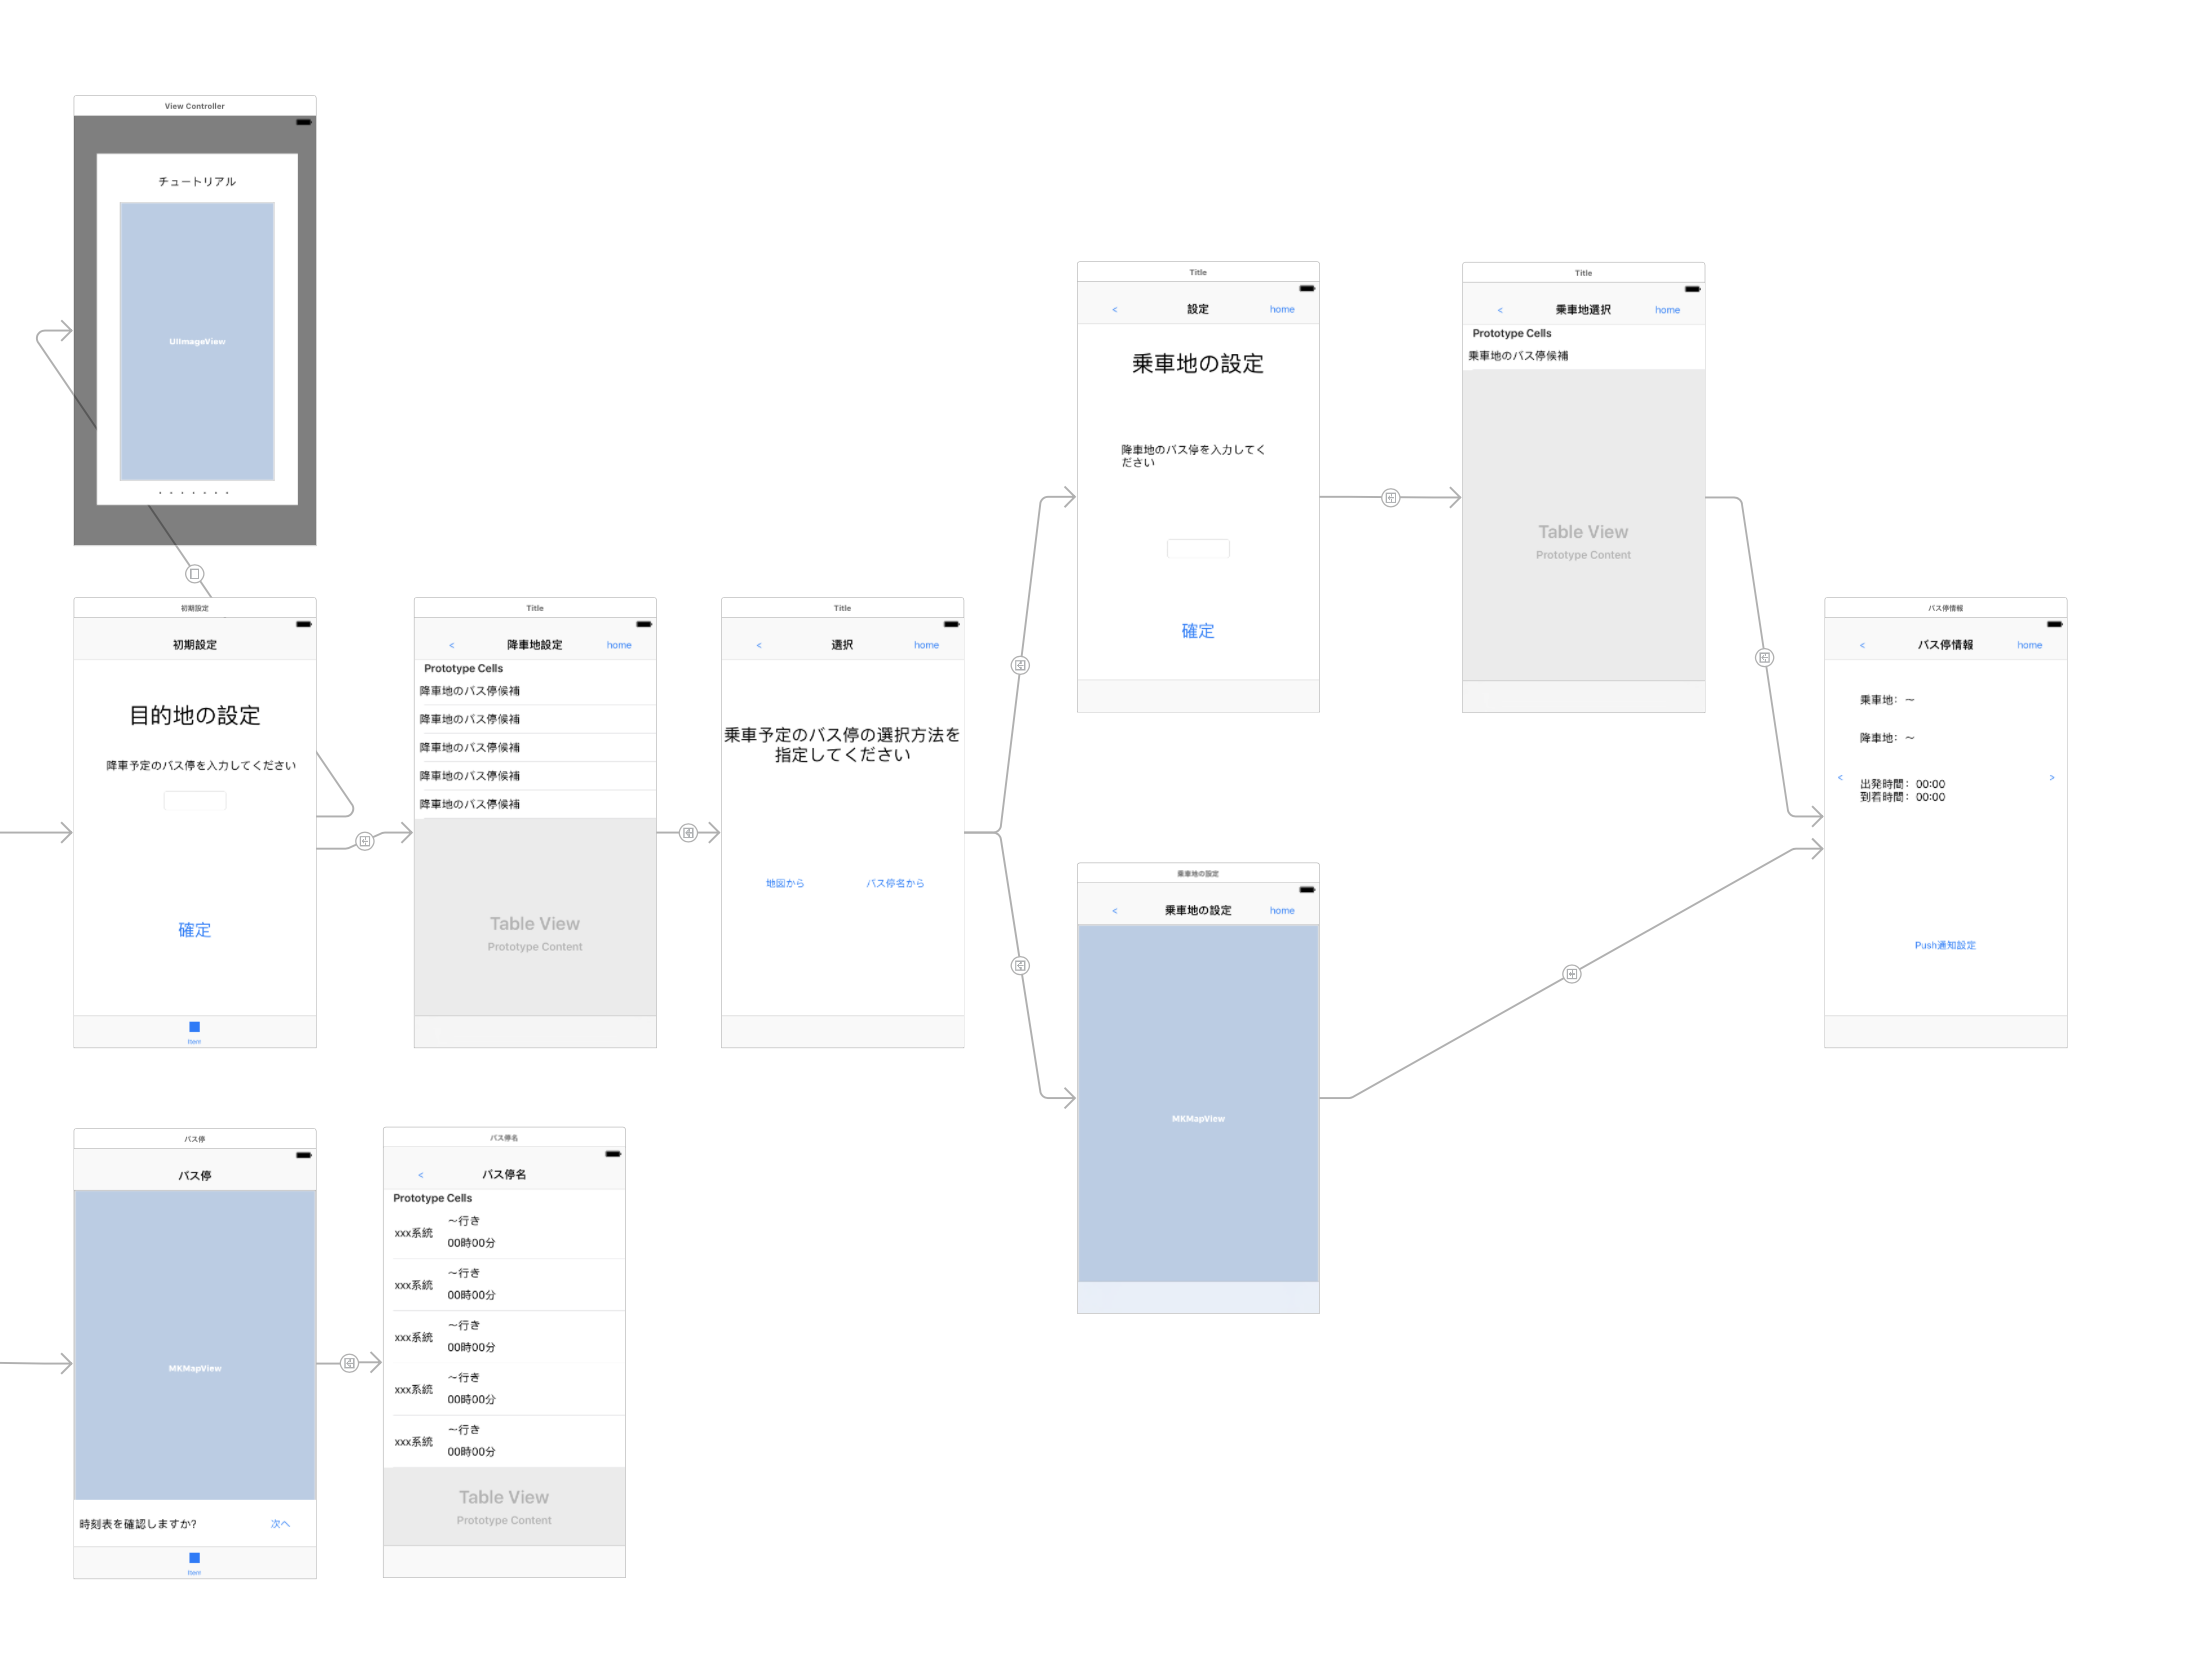
\includegraphics[clip,width=19cm,angle=90]{img/picture.png}
    \label{fig:senni}
  \end{center}
\end{figure}

\chapter{中間発表ポスター}
\begin{figure}[htbp]
  \begin{center}
    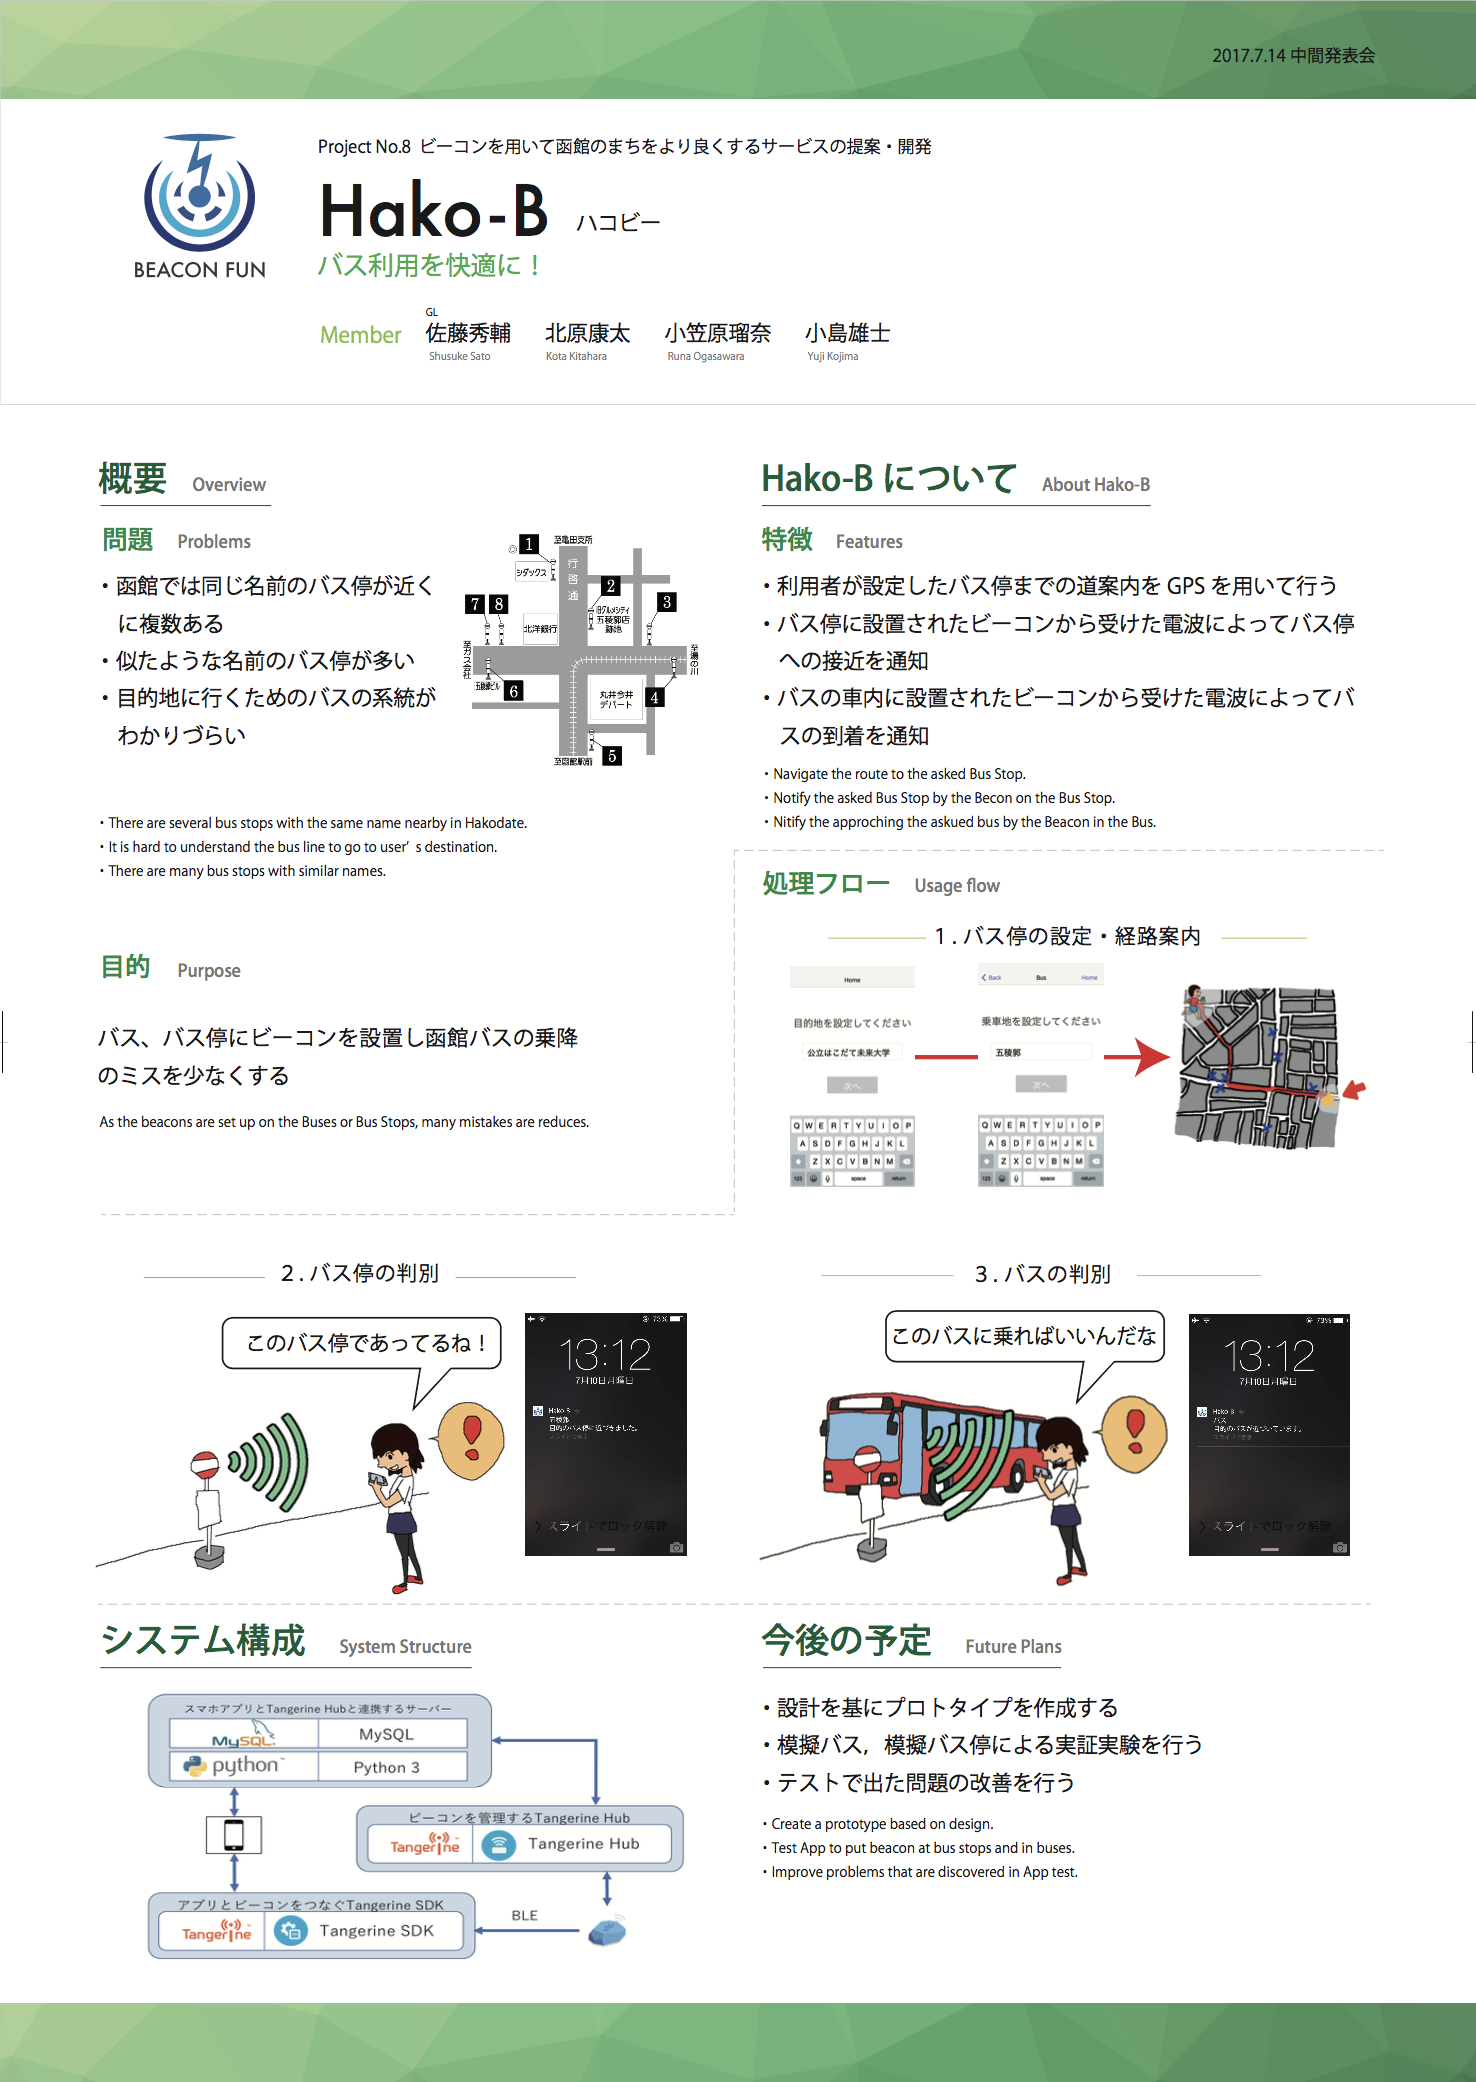
\includegraphics[clip,width=14cm]{img/poster.png}
    \label{fig:poster}
  \end{center}
\end{figure}

  \chapter{最終成果報告会で使用した本グループのポスター}
  
  %付録の終わり
  \end{appendix}
  
  
  %\backmatter
  
  \begin{thebibliography}{9}
    \bibitem{JohoWhitepaper} 総務省, 平成28年版 情報通信白書 第1部 特集 IoT・ビッグデータ・AI~ネットワークとデータが創造する新たな価値~
    http://www.soumu.go.jp/johotsusintokei/whitepaper/ja/h28/html/nc122530.html
  
    [last accessed 2017/7/24]
  \end{thebibliography}
  
  \end{document}
  